\documentclass{article}

\usepackage{todonotes}
\usepackage{hyperref}
\usepackage{fancyhdr}

\pagestyle{fancy}
\rhead{Document number: RBB4-01}

\graphicspath{{img/}}

\begin{document}
\title{Minor Change}
\author{}
\date{}
\maketitle

\section{Change design description}
Design title: Installation of a transponder

\section{Aircraft identification}
\begin{tabular}{|l|l|}
\hline
Aircraft type & Serial Number \\
\hline
Pilatus B4 & All \\
Pilatus B4A & All \\
Pilatus B4AF & All \\
\hline
\end{tabular}

\section{Design summary}
This change is made to install a TSO-approved Mode-S transponder (like for example the Garrecht VT-01 UltraCompact) with a transflex-4 antenna in the applicable aircraft. The design covers the installation of an antenna, a transponder and wiring. This change is identical for all effective aircraft.

\section{Applicable requirements}
\begin{tabular}{|l|p{10cm}|}
\hline
Identification & Title \\
\hline
CS 22.1301 &  Equipment/Function and installation \\
CS 22.1353 &  Electrical Systems and Equipment/Storage battery design and installation \\
CS 22.1365 &  Electrical Systems and Equipment/Electric cables and equipment \\
CS 22.1431 &  Miscellaneous Equipment/ATC airborne equipment \\
EuroCAE ED-73B & Minimum operational performance specifications for secondary surveillance radar mode s transponders \\
\hline
\end{tabular}

\section{Minor/Major classification}
The change has no appreciable effect on the mass, balance, structural strength, reliability, operational characteristics, noise, fuel venting, exhaust emission, or other characteristics affecting the airworthiness of this product. Therefore, this change can be considered Minor.

\section{Weigth and balance}
After the change has been performed, a new weight \& balance report must be made. This can be performed by either weighing of the aircraft of by calculation.

\section{Substantiation of the requirements}
\begin{tabular}{|l|p{10cm}|}
\hline
Requirement & Substantiation \\
\hline
CS 22.1301 (b) & The transponder will be installed in the instrument panel of the aircraft according to the instructions of the manufacturer of the transponder. \\
\hline
CS 22.1301 (b) & The antenna will be installed through a small hole in the fuselage, and will be fixated to the fuselage. The copper ground-block of the antenna is replaced with a aluminium ground-plate, thus preventing potential contact-corrosion. (See appendix 1, tekening/foto) \\
\hline
CS 22.1301 (b) & The cable and wires used will be installed according to the instructions of the manufacterer of the transponder. The antenna cable type will be chosen according to the instructions of the manufacturer of the transponder. \\
\hline
CS 22.1365 (a) & The transponder will be connected to the electrical system according to the instructions of the manufacturer of the transponder. \\
\hline
CS 22.1365 (b) & Overload protection will be installed according to the instruction of the manufacturer of the transponder. \\
\hline
CS 22.1431 (a) & This Minor change is only valid for TSO-approved transponders. For example, the Garrecht VT-01 UltraCompact is ETSO 2C112a approved. \\
\hline
CS 22.1431 (b) & The control devices are all accessible on the instrument panel. Sufficient cooling is accomplished when installing the transponder according to the instructions of its manufacturer. \\
\hline
EuroCAE ED-73B & After the change is performed, the transponder will be tested in accordance with the instructions of the manufacturer of the transponder in order to verify that the transponder is in compliance with the EuroCAE ED-73B requirements. \\
\hline
\end{tabular}


Note:
All installation work will be performed in accordance with acceptable methods, techniques and practices for alternations, inspections and repair as shown in FAA documents AC 43.13.B and AC 43.13-2A and the installation manual of the transponder in question.

\section{Attached appendices}
\begin{enumerate}
\item Appendix A: Tekening/foto van de antenne.
\end{enumerate}

\begin{figure}

\includegraphics[width=\textwidth,keepaspectratio]{antenna_location}
\caption{A sketch of the antenna location, relative to Spant 4 and the gear area.}
\label{fig:antenna_location}
\end{figure}


\begin{figure}
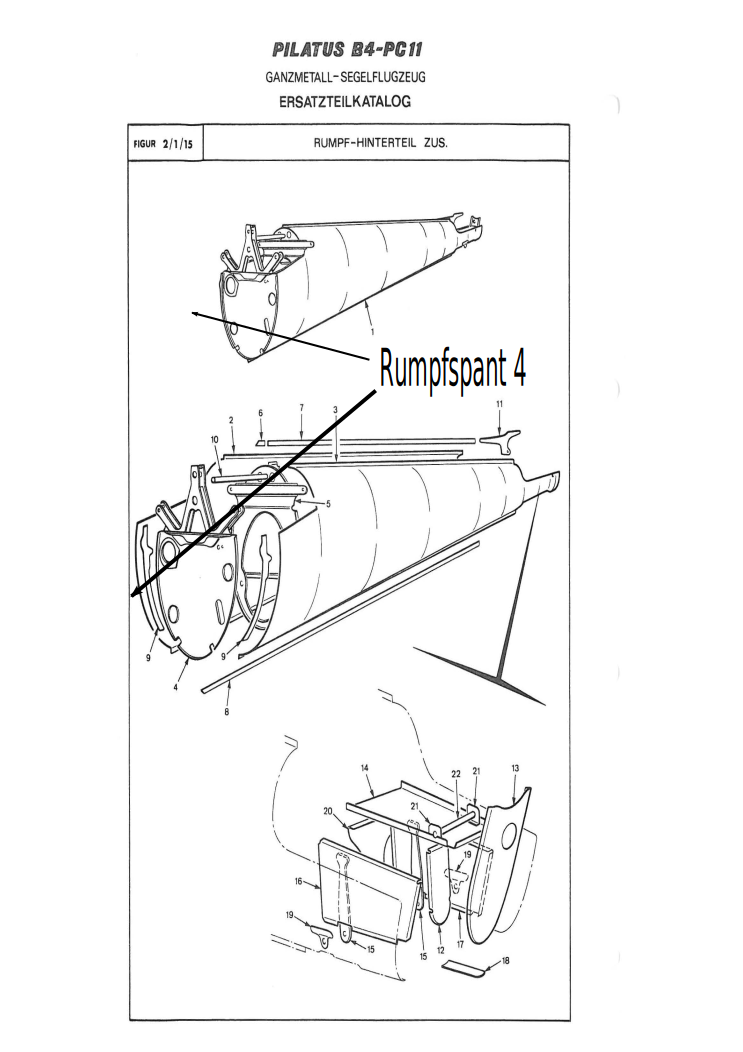
\includegraphics[width=\textwidth,keepaspectratio]{b4_ersatzteil_katalog_fig_2_1_15_annotated}
\caption{Figure 2/1/15 from the Pilatus B4 ersatzteil katalog, with Rumpfspant 4 (referenced in Figure \ref{fig:antenna_location}) pointed out.}
\label{fig:ersatzteil_rumpfspant4}
\end{figure}

\begin{figure}
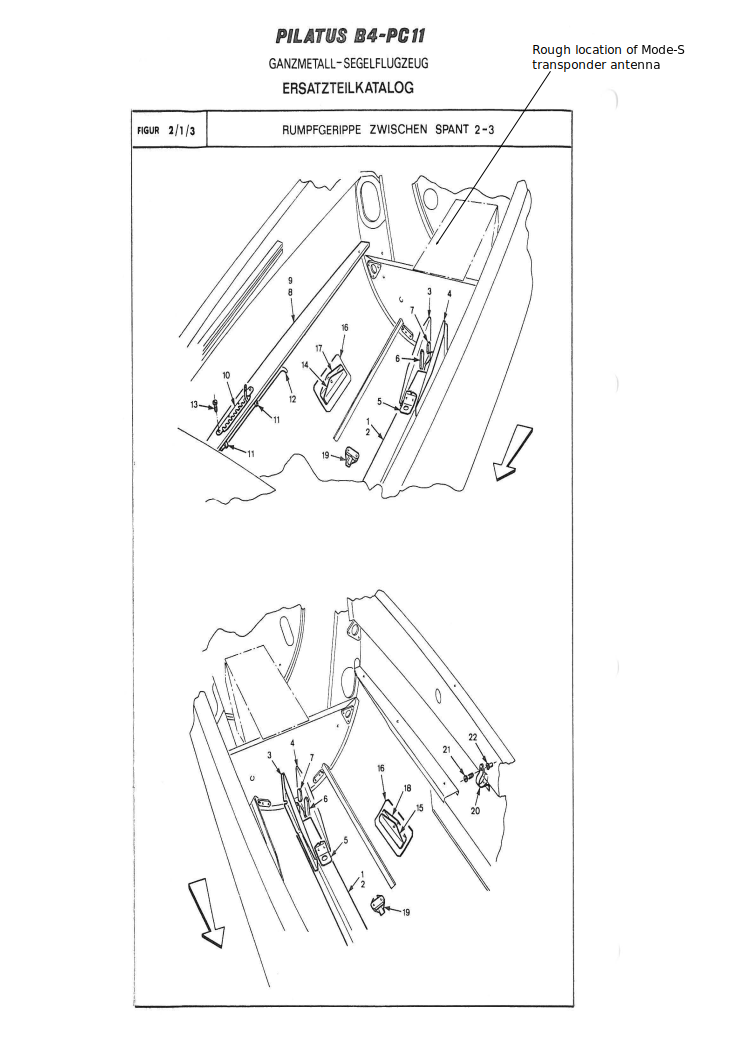
\includegraphics[width=\textwidth,keepaspectratio]{b4_ersatzteil_katalog_fig_2_1_3_annotated}
\caption{Figure 2/1/3 from the Pilatus B4 ersatzteil katalog, with the location of the antenna pointed out.}
\label{fig:ersatzteil_antenna}
\end{figure}

\begin{figure}
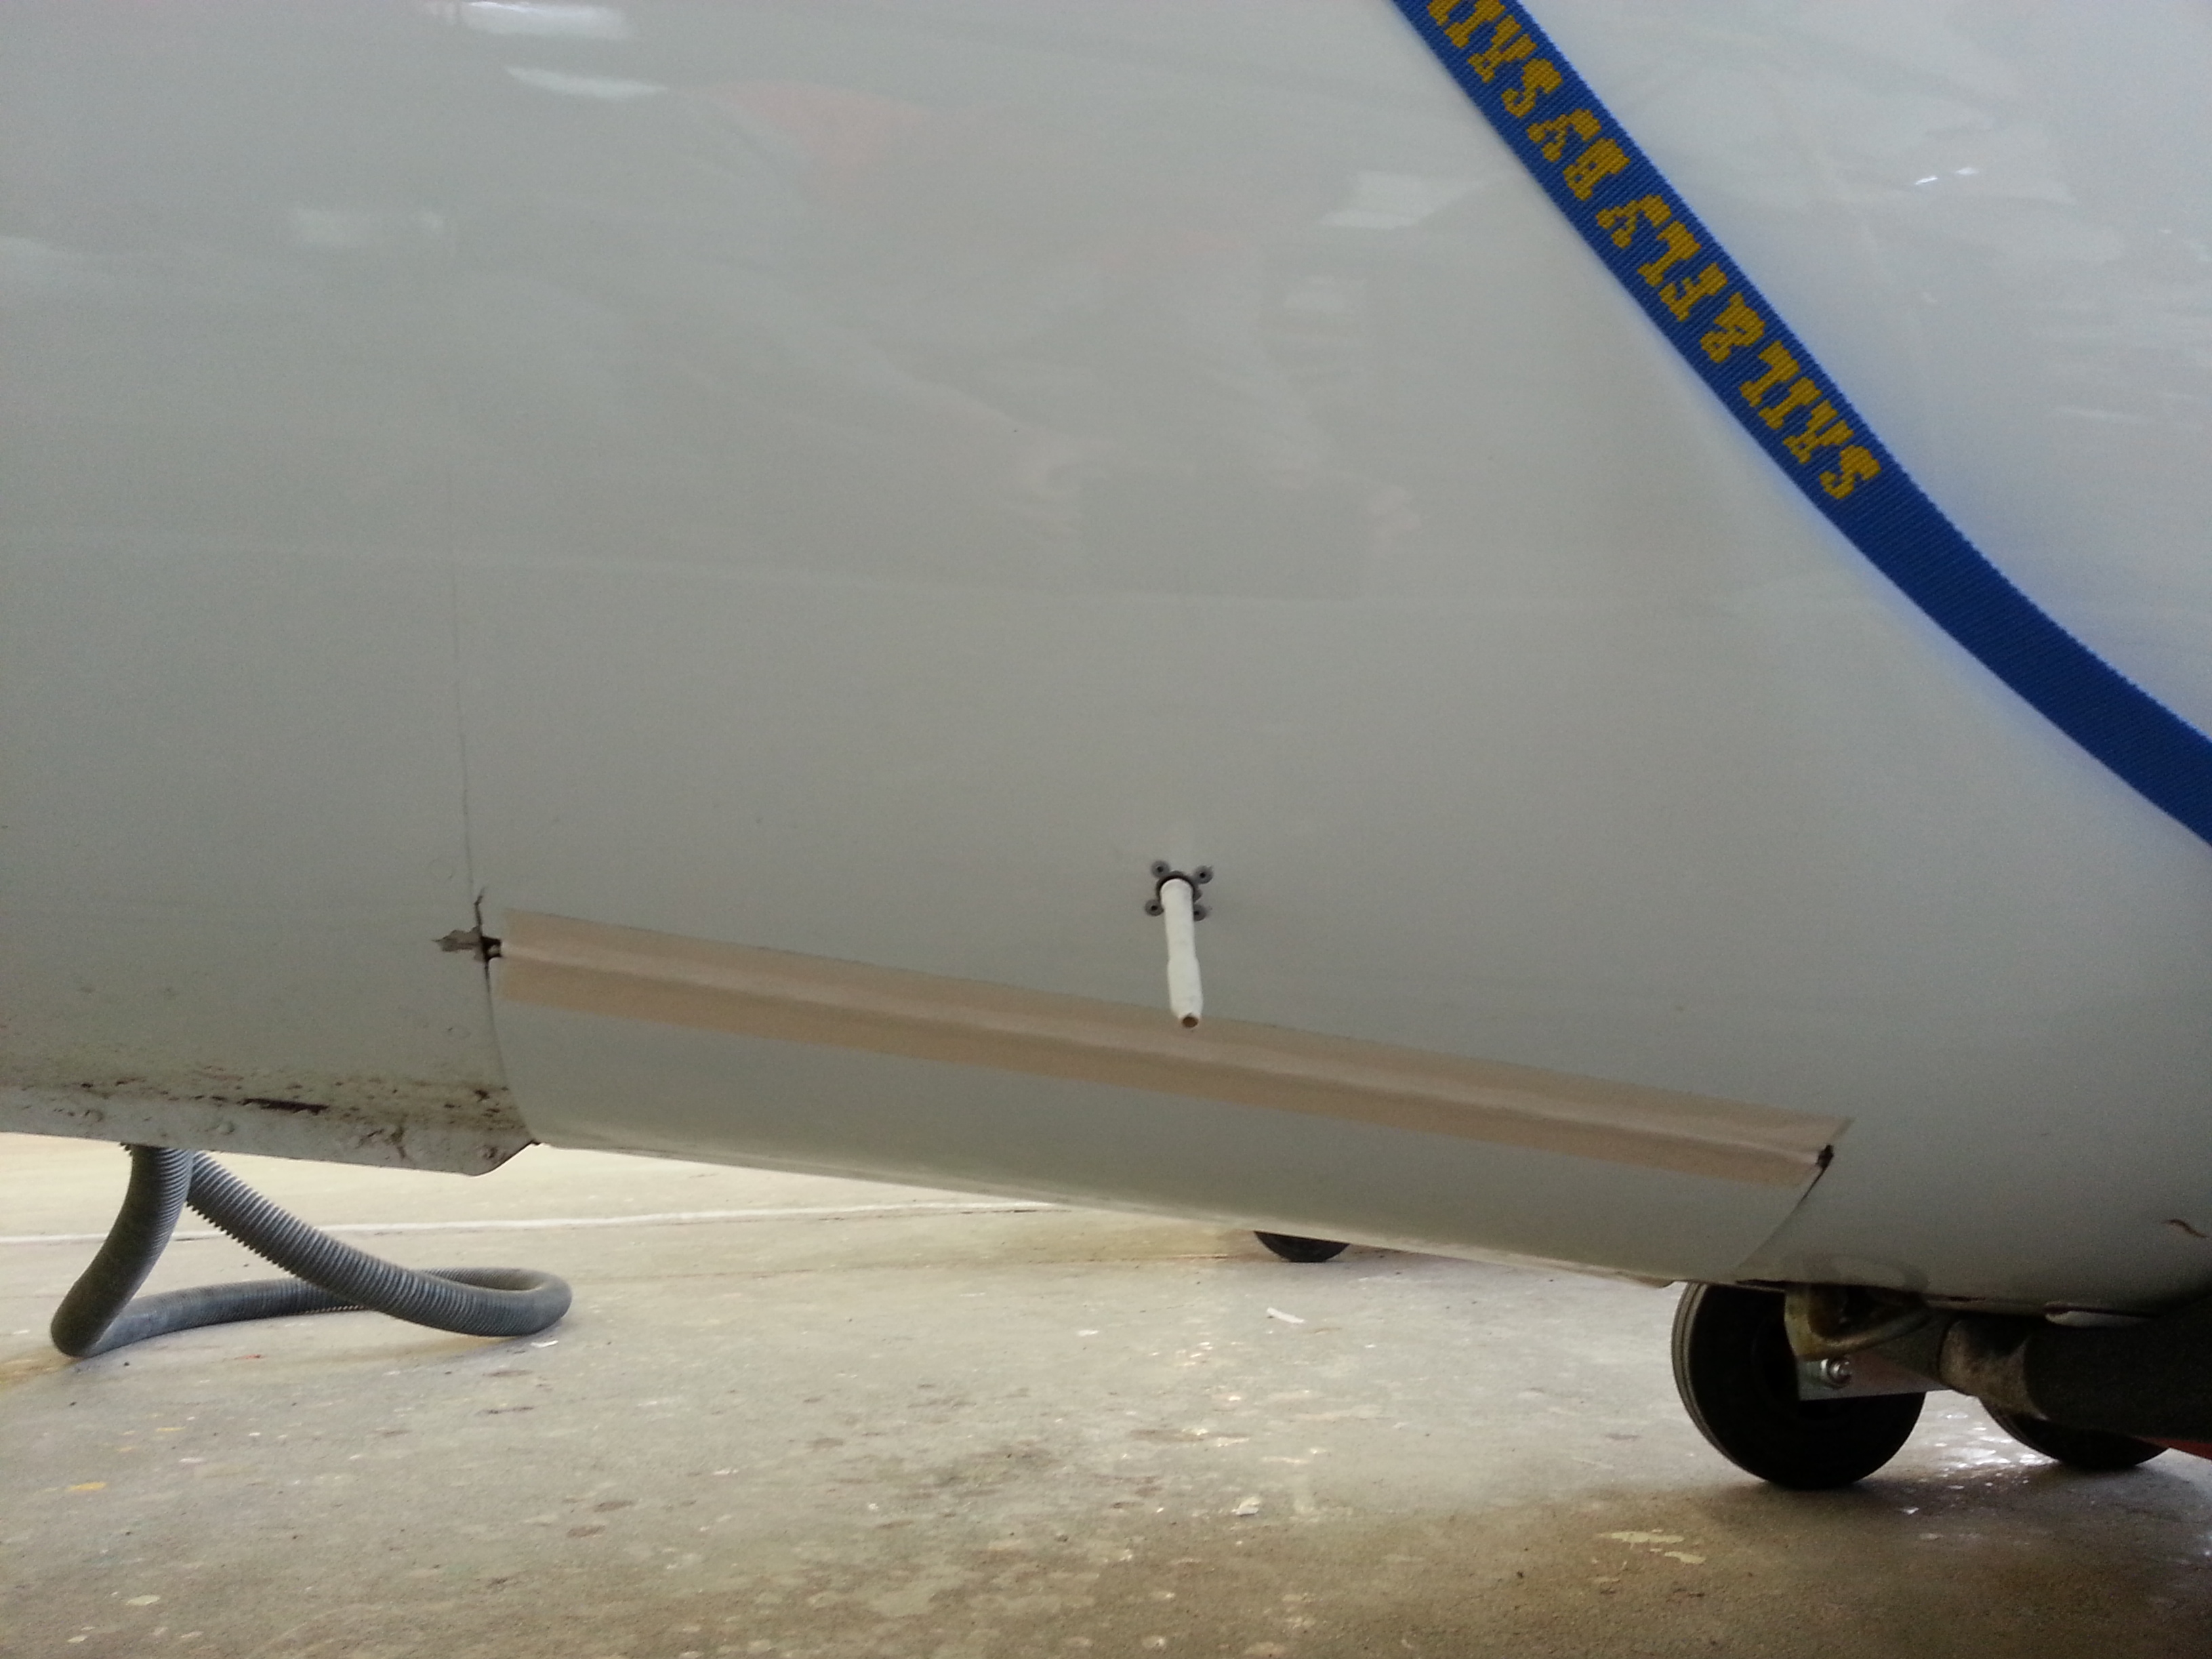
\includegraphics[width=\textwidth,keepaspectratio]{outside}
\caption{A photograph, taken from the outside of the fuselage, of the antenna installed. Note the four rivets used to mount the antenna to the fuselage plating.}
\label{fig:outside}
\end{figure}

\begin{figure}
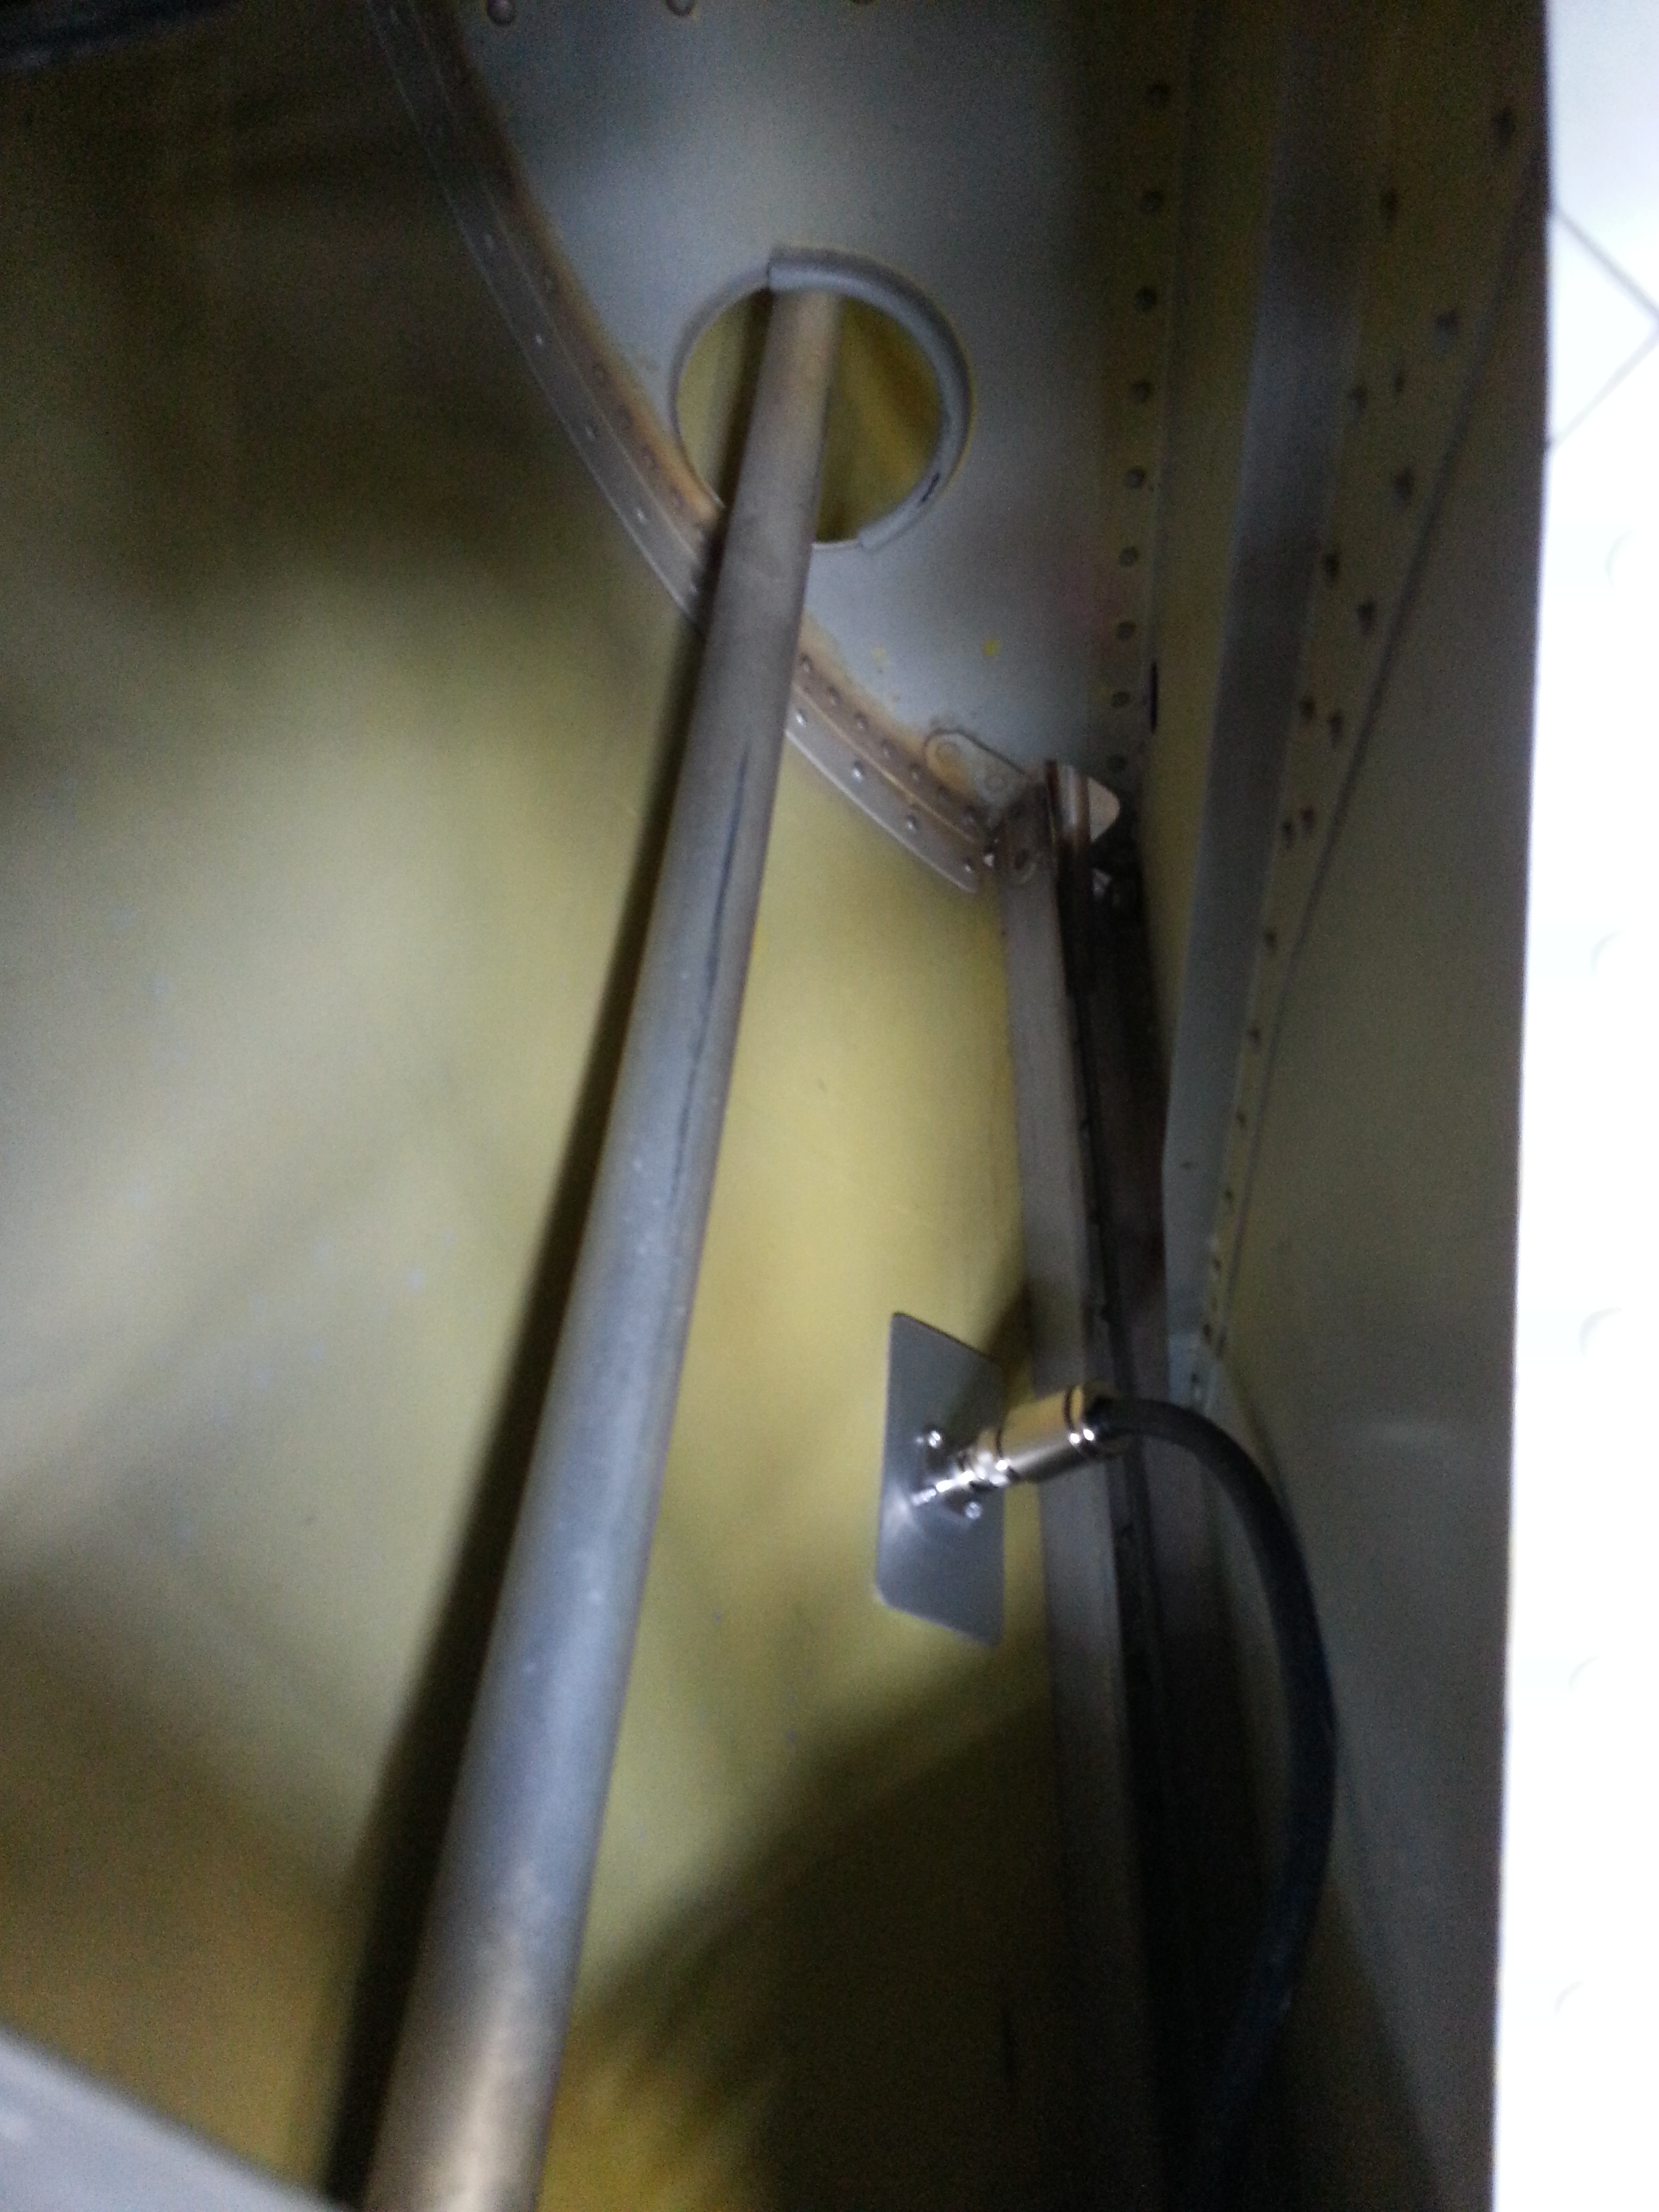
\includegraphics[width=\textwidth,keepaspectratio]{inside}
\caption{A photograph, taken from the inside of the fuselage, of the antenna installed. Note the aluminium plating, which replaced the original copper block. Replacement was necessary in order to prevent contact-corrosion.}
\label{fig:outside}
\end{figure}

\end{document}
